\chapter{Introduction}
\label{ch:introduction}

\dictum[Kir Bulychev,\\Alice on Alive Planet ]{%

\begin{otherlanguage}{russian}
Есть такое наблюдение: если насморк не лечить, то он пройдет через неделю, а если лечить, то через семь дней.
\end{otherlanguage}

There's a following observation: if you don't treat the cold, it will pass in  week, but if you do, then it will pass in seven days.

}%
\vskip 1em

\textit{In silico} modelling allows to examine an array of parameters and possibilities which would be difficult or impossible to characterise using traditional research methods \cite{colquitt2011silico}. Such flexibility allows the pursuit of two competing goals: to gain a new understanding of the system from the available knowledge, and to use available data to predict future progression of the system in question \cite{nguyen2016analysis}.

The recent example of COVID-19 pandemic brought to the light some of the viral \textit{in silico} modelling techniques. Amino-acid sequence based molecular modelling uses existing knowledge of protein folding to predict conformations of spike glycoproteins \cite{vankadari2020emerging} and their docking sites \cite{hall2020search}. Dynamic infection modelling primarily focuses on the second goal - assisting public health decisions by describing viral transmission, for example, by estimating case mortality \cite{anastassopoulou2020data}, or potential effectiveness of social policies \cite{giordano2020modelling}. Such applications of \textit{in silico} modelling make sense due to the time sensitive nature of a global pandemic, a novel under-researched pathogen, and existing limitations in data reporting.

Influenza is another viral pandemic threat \cite{sutton2018pandemic, taubenberger20191918}. However, unlike COVID-19, influenza has been extensively studied over the last 100 years, and we have lots of protein structure \cite{calder2010structural}, function \cite{pinto2006m2, lamb2001death}, and host interaction \cite{zhao2017influenza} information available. Despite this dearth of knowledge, influenza models still often use small datasets with few observed variables to fit a small model of infection \cite{smith2011influenza}, which are rarely examined under other experimental conditions \cite{dobrovolny2013assessing}. While there is a certain benefit to the use of tractable and easily understandable models, their minimalist structure doesn't allow for inference on specific molecular targets for intervention \cite{heldt2013multiscale}.

Attempts to introduce additional knowledge of underlying intracellular processes \cite{heldt2013multiscale, rudiger2019multiscale} often end up with models which may describe influenza infections in a bigger variety of experimental conditions, but also rely on many unobserved quantities and variables.

Ultimately, the struggle boils down to the problem all multiscale models face \cite{qu2011multi} - hierarchical organization of systems is an artifact of our ability to observe them. In a process of mathematical modelling we need to bridge these apparent gaps between observed spatial and temporal scales, while preserving the relevant detail, which makes the inclusion of smaller scales important.

In this work, we attempt to provide a case study for how such challenges can be approached. We use small scale models to answer specific questions about influenza infection, and then use approximated predictions made by those small scale models to make judgements about larger scale outcomes. This approach can, perhaps, be conceptualized as a "matryoshka" (Russian nesting doll): each individual doll can be used separately, but together they introduce the user to new concepts and experiences which a single doll would not able to represent sufficiently.

\section{Influenza Virus Burden}

In 2004 acute lower respiratory infections (ALRI) were second leading cause of disease (429.2 million cases), and third leading cause of death worldwide \cite{world2008global} (4.2 million deaths). ALRI can be caused by a variety of pathogens, such as influenza virus, rhinovirus, coronavirus, respiratory syncytial virus and others. Previously, influenza virus was reported as the second most common pathogen identified in children with ALRI \cite{nair2011global}.

Worldwide, influenza virus infections result in large direct healthcare costs, indirect loss of productivity costs \cite{de2015systematic}, and heavy disease burden, projected to cost \$87.1 billion \cite{molinari2007annual}. World Health Organization (WHO) estimates that influenza virus leads to 3-5 million cases of severe illness, and about 290,000-650,000 respiratory deaths annually \cite{influenza_seasonal_2018}.

Influenza infection poses greater risk for pregnant women, young children, the elderly, and individuals with chronic and immunosuppressive medical conditions. Due to workplace exposure, health care workers are at high risk for getting ill and further transmitting influenza to vulnerable individuals \cite{influenza_seasonal_2018}.

\section{Influenza Virus Structure}

Influenza viruses are negative sense ribonucleic acid (RNA) viruses of the family Orthomyxoviridae \cite{Orthomyxoviridae2011}.

Influenza virus genomic RNA is packaged with protective nucleoprotein together with polymerase complexes. Influenza viruses carry eight unique viral RNA strands, packaged into ribonucleoprotein  (vRNP) segments (Table \ref{table:fluSegments} \cite{das2010structures, dubois2014influenza}). Through use of alternative mRNA splicing influenza A may encodes up to 17 known proteins.

Electron microscopy and single‑molecule fluorescence in situ hybridization studies provide evidence for selective packaging over random inclusion of the eight vRNP segments \cite{eisfeld2015centre}. However, there's a growing awareness that semi-infectious viral particles, which lack full set of vRNPs are also contributing towards viral infectivity.

Packaged vRNPs are protected by capsid layer consisting mostly of matrix protein M1. This layer embeds ion channel M2, and transmembrane segments of haemagglutinin (HA) and neuraminidase (NA) spikes. On the outside, capsid layer is covered with a protective lipid bilayer taken from the virus producing host cell during the packaging and detachment process.

Three largest vRNP segments - PB2, PB1, and PA - encode polymerase subunits, responsible for viral RNA synthesis in the host cell nucleus.

Intermediate sized segments encode nucleoprotein (NP), which protects viral RNA strands, and two surface glycoprotein spikes HA and NA. HA spike binds host cell-surface sialic acid receptors initiating viral entry. NA spike on the other hand cleaves sialic acid residues from the new viral particles, to release them from the host cell.

Based on these glycoprotein spikes, influenza A viruses are categorized into antigenic subtypes. 18 HA and and 11 NA subtypes (named H1-18 and N1-11, respectively) have been identified so far \cite{InfluenzaAAntigenicSubtypes}. Thus, for example H3N2 virus contains a H3 subtype HA and a N2 subtype NA.

Segment M encodes influenza matrix protein M1 which forms a protective capsid layer around vRNPs. Open reading frame shift during translation leads to production of ion channel protein M2, based on the same segment \cite{dubois2014influenza}.

Finally, smallest segment NS encodes several non-structural proteins which assist the course of infection.

Influenza virus particles often carry host proteins, which they "borrow" from their host cell. Some of these host proteins, such as annexin A2, $\beta$-actin, and ubiquitin B are present in the virions in amounts exceeding native viral proteins NS1, M2, and NEP \cite{hutchinson2014conserved}. Currently, it is unclear whether those host proteins carry provide any significant function during infection, or their presence is simply an artifact of viruses subverting cellular microvesicle formation pathways to produce enveloped virions \cite{hutchinson2014conserved}.

\begin{table}[h!]
\centering
\caption{Influenza virus vRNP segments}
\label{table:fluSegments}

\begin{tabular}{p{2cm} p{10cm}}
\hline 
\textbf{Segment}&    \textbf{Protein}\\
\hline
PB2&    polymerase subunit PB2\\
\hline
PB1&    \tabitem polymerase subunit PB1\\
   &    \tabitem protein PB1-F2, which has apoptotic function\\
   &    \tabitem protein PB1-N40 \cite{dubois2014influenza}\\
\hline
PA&     \tabitem polymerase subunit PA\\
  &     \tabitem protein PA-X, which regulates host translation shutoff \cite{khaperskyy2016selective}\\
  &     \tabitem protein PA-N155 \cite{dubois2014influenza}\\
  &     \tabitem protein PA-N182 \cite{dubois2014influenza}\\
\hline
HA&     haemagglutinin, which binds to the host cell-surface sialic acid receptors\\
\hline
NP&     nucleoprotein, which encapsidates the viral single-stranded RNAs\\
\hline
NA&     neuraminidase, which cleaves sialic acid residues from the new viral particles, releasing them from the host cell\\
\hline
M&      \tabitem matrix protein M1\\
 &      \tabitem ion channel M2\\
 &      \tabitem protein M42 \cite{dubois2014influenza}\\
\hline
NS&     \tabitem non-structural protein NS1A, which suppresses host mRNA production\\
  &     \tabitem nuclear export protein NS2/NEP\\
  &     \tabitem protein NS3 \cite{dubois2014influenza}\\
\hline
\end{tabular}
\end{table}

\section{Influenza Infection}

Figure \ref{figure:fluInfectionStages} provides a simplified schematic representation of influenza infection progression in host respiratory cells. First, the influenza virus attaches to the cell membrane by presenting viral HA cell-surface sialic acid receptors. This triggers formation of the transport endosome.

A change of pH during endosomal transport sends a signal through the M2 ion channel of influenza, triggering virion uncoating, which includes the formation of the fusion pore and dissolving bonds between M1 proteins. Viral uncoating is a complex process which is reported to involve host cell proteins \cite{banerjee2014influenza}.

Released genetic material then migrates to cell nucleus, starting replication of viral RNA, which in turn initiates the synthesis of viral proteins. Newly synthetized proteins assemble into virions at the cell membrane and exit from the host cell.

\begin{center}
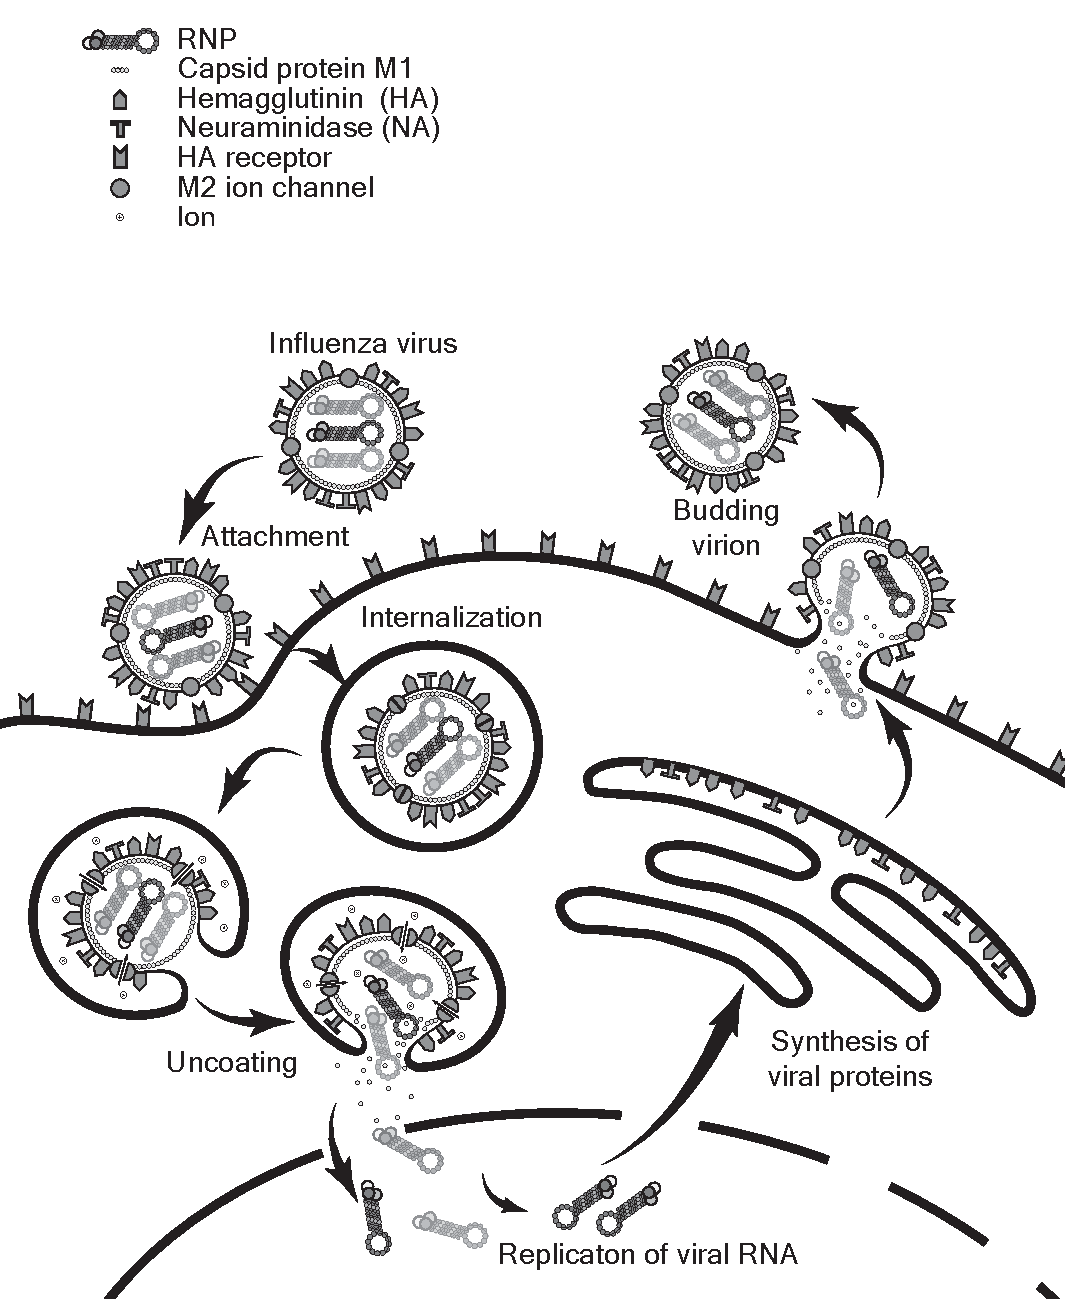
\includegraphics[width=0.95\textwidth, trim={0cm 0cm 0cm 0cm}, clip]{D_chapters/0_introduction/flu_stages.pdf}
\captionof{figure}{Influenza virus infection course}
\label{figure:fluInfectionStages}
\end{center}

\section{Influenza Infection Prevention and Treatment}

Preventative measures, such as annual vaccination, hand washing, respiratory hygiene, and post exposure self-isolation are the best available measures in mitigating influenza infection risks \cite{influenza_seasonal_2018}.

Influenza vaccine formulation, recommended by WHO commonly includes \cite{RecommendedCompositionVaccines}

\begin{itemize}
    \item one H1N1 influenza A virus,
    \item one H3N2 influenza A virus,
    \item one or two influenza B viruses.
\end{itemize}

The influenza vaccine provides immunity to healthy adults even when the formulation is not perfectly matched to circulating virus strains, but vaccination is especially important for individuals in high risk groups.

Likewise, in cases where disease occurs, for healthy adults WHO suggests symptomatic treatment and social distancing. For high risk groups the use of antiviral drugs is recommended \cite{influenza_seasonal_2018}. So far, two main classes of antiviral drugs against influenza have been developed (Figure \ref{figure:fluDrugs}).

Adamantane type drugs, such as amantadine, bind to the M2 ion channel, preventing endosomal acidification, which inhibits virus uncoating. In 2011 WHO reported that the majority of circulating influenza A viruses are resistant to this type of drug \cite{whoAntivirals2011}. WHO no longer recommends adamantanes for use \cite{influenza_seasonal_2018}.

\begin{sidewaysfigure}
\begin{center}
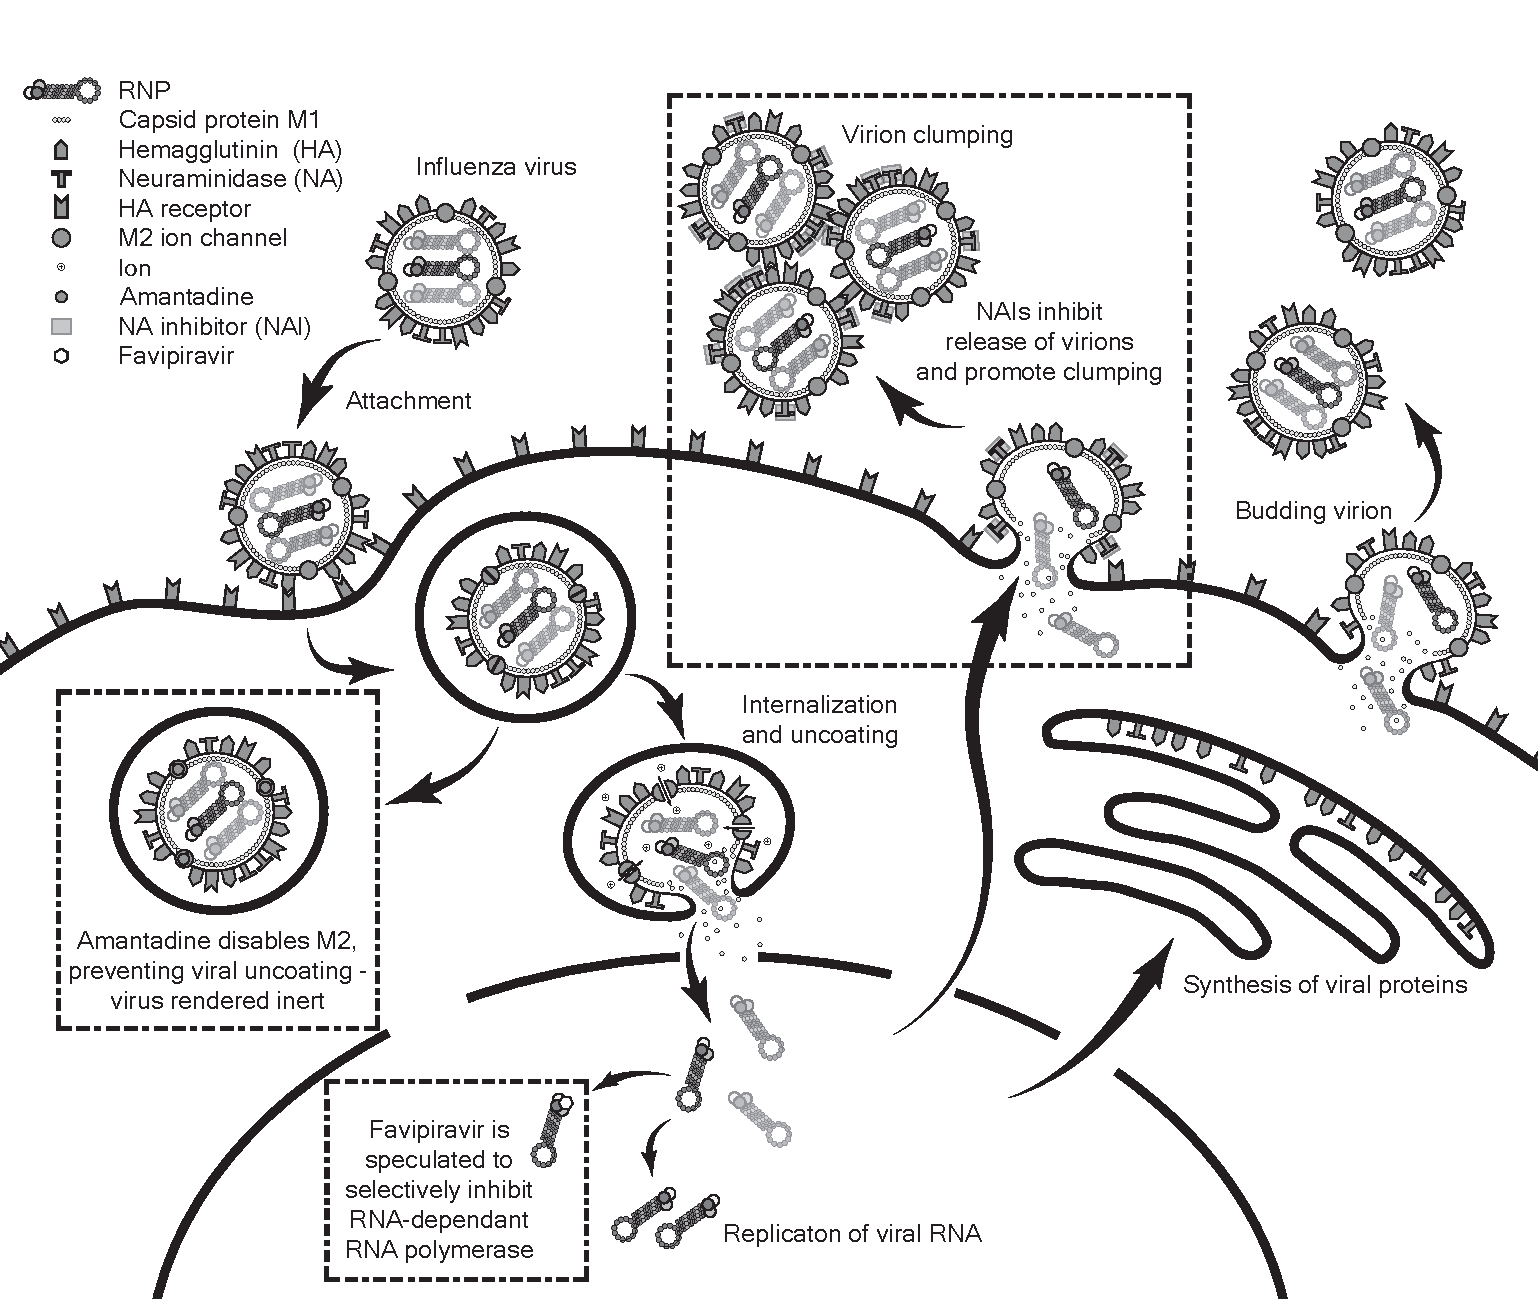
\includegraphics[width=0.75\textwidth, trim={0cm 0cm 0cm 0cm}, clip]{D_chapters/0_introduction/flu_drug.pdf}
\captionof{figure}{Mechanism of action of influenza antiviral drugs. Adapted from \cite{stiver2003treatment}.}
\label{figure:fluDrugs}
\end{center}
\end{sidewaysfigure}

Neuraminidase inhibitors bind to the viral surface enzyme neuraminidase and prevent cell surface receptor cleavage, inhibiting new virions' escape from infected cells. 2016-2017 survey reported that only about 0.2\% of collected influenza viruses showed resistance to one or more type of neuraminidase inhibitors \cite{lackenby2018global}. This type of drug remains suitable for use in the clinic, but emerging resistance makes continued monitoring necessary.

Additionally, favipiravir is a broad spectrum antiviral drug, which acts as a chain terminator at the site of viral RNA incorporation \cite{shiraki2020favipiravir}. Wide applicability to a variety of viruses often comes with concerns of cellular toxicity. Favipiravir has been approved as an emergency treatment for novel (rather than seasonal) influenza viruses in Japan in 2014, however wider approval is delayed in part due to potential teratogenic concerns.


\section{Host directed anti‐viral strategies}

Currently available influenza drugs  target viral proteins M2 and NA. This approach allows for a specific mechanism of action, which, ideally, should not interfere with host cellular systems.

One significant problem with this approach is that, by introducing the antiviral drugs into the clinic, we exert evolutionary pressure on the virus. In turn, through the process of antigentic drift the virus may modify its target protein to escape inhibition by the drug, rendering the drug useless (e.g. adamantanes).

These concerns over antiviral drug resistance, and growing awareness of host proteins involvement in successful infection led to the emergence of a new drug development approach. Instead of targeting a viral protein, we try to target a host cell protein involved in viral infection. Thus, we can inhibit infection without subjecting the virus to direct selection.

\begin{figure}
\begin{center}
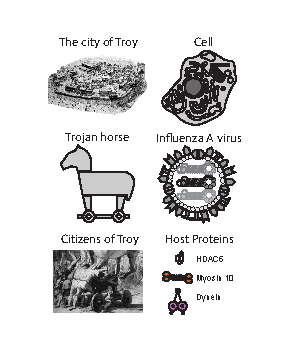
\includegraphics[width=0.7\textwidth, trim={0.6cm 0.6cm 0.6cm 0.6cm}, clip]{D_chapters/0_introduction/flu_troy.pdf}
\caption[Trojan siege metaphor for host directed anti-viral strategies]%
{Trojan siege metaphor for host directed anti-viral strategies. \par The city of Troy is a black and white render of reconstruction of the Homeric city of Troy, Turkey. (Photo by DeAgostini/Getty Images). The citizens of Troy are a black and white crop of "The Procession of the Trojan Horse into Troy from Two Sketches Depicting the Trojan Horse", oil on canvas by Giovanni Domenico Tiepolo, c. 1760 in the National Gallery, London.}
\label{figure:fluTroy}
\end{center}
\end{figure}

Conceptually such an approach can be understood through the story of a Trojan siege (Figure \ref{figure:fluTroy}). Much like a Trojan horse, which could not make it inside the city without the help of its citizens, viruses require host protein help for successful infection. Choosing to target these host proteins in an antiviral treatment is alike to convincing the Trojans to leave the horse at the door.

A major challenge in host directed anti‐viral strategies is cellular toxicity (which, however, is not exclusive to this approach). It is a complex issue, which we believe is best addressed by interrogating systemically the involvement of the protein in both cellular and viral processes, as well as elucidating the specific mechanism of action of a drug-like agent.

\section{HDAC6 Structure and Function}

Histone deacetylases are a class of enzymes that remove acetyl groups from chromatin and other acetylated proteins. Currently 18 HDAC proteins are known, which are classified into 4 classes. HDAC6 belongs to IIb class, which is primarily localized in the cytoplasm \cite{hai2016histone}.

Among other histone deacetylases HDAC6 is the only one to carry tandem catalytic domains CD1 and CD2 (Figure \ref{figure:HDAC6Domains}). Dynein motor binding (DMB) domain is located between them. HDAC6 also has a ubiquitin-binding domain ZnF ("zinc-finger") which senses polyubiquitinated misfolded protein cargo \cite{hai2016histone}. HDAC6-ZnF selectively binds to ubiquitin chains having unanchored C terminal diglycine \cite{ouyang2012protein} with a very high affinity \cite{zhang2008mice}.

\begin{center}
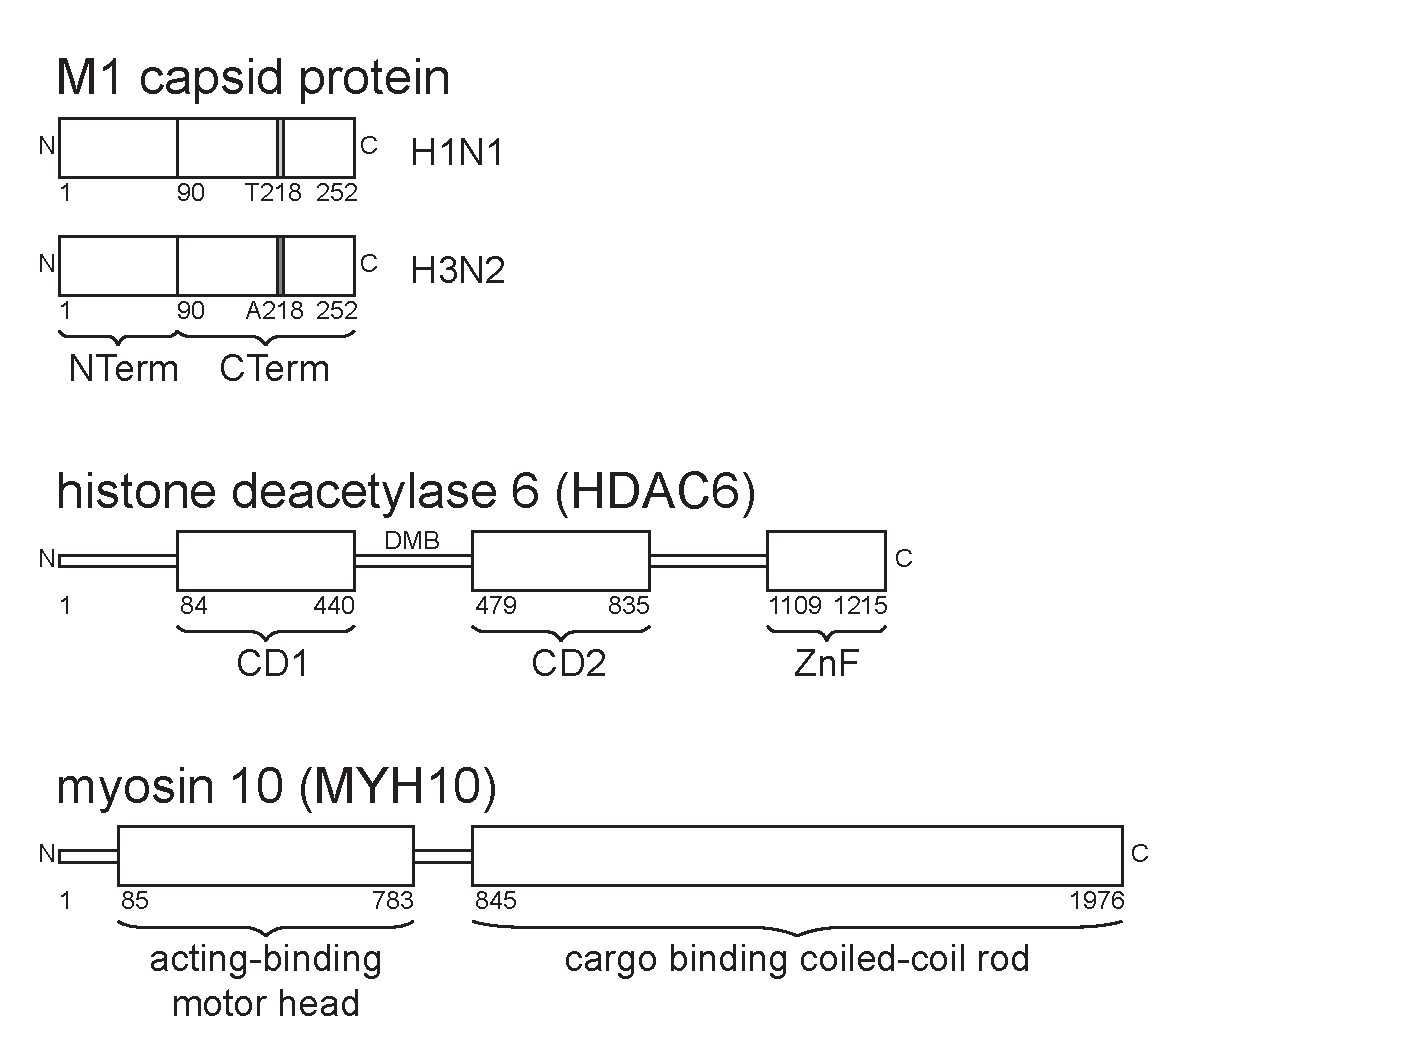
\includegraphics[width=1\textwidth, trim={0cm 6cm 8cm 8.8cm}, clip]{D_chapters/0_introduction/protein_domains.pdf}
\captionof{figure}{HDAC6 domain organization}
\label{figure:HDAC6Domains}
\end{center}

HDAC6 deacetylates tubulin \cite{zhang2003hdac, zhang2008mice} (polymer making up the microtubules), and heat shock protein 90 (Hsp90) \cite{kovacs2005hdac6} (a chaperone protein which assists protein folding and degradation). HDAC6 senses ubiquitinated protein aggregates and triggers their clearance \cite{boyault2007hdac6}. HCAC6 also assists in stress granule formation and cellular oxidative stress recovery \cite{kwon2007deacetylase}.

During influenza infection, HDAC6 (specifically, HDAC6-ZnF) and other components of aggresome processing machinery - molecular motors myosin 10 and dynein - were essential for efficient uncoating. Involvement of molecular motors suggested that influenza uncoating is achieved through physical forces generated by microtubule- and actin-associated motors \cite{banerjee2014influenza}.



\section{Mathematical models allow functional analysis of biological systems}

A variety of mechanistic mathematical modelling approaches has been used to analyze and elucidate function of cellular systems and viral infections.

For example, a process through which molecular motors may exert force onto influenza virus capsid layer is called tug-of-war. Tug-of-war involves velocity and force balance between all involved parties. Previously it has been used to describe two types of microtubule motors to model endosomal transport \cite{muller2008tug}, and to prove that competitive and cooperative modes of molecular motor transport are not mutually exclusive.

A stochastic model of bidirectional microtubular transport \cite{gazzola2009stochastic} is used to describe transport of adenovirus, and allows to predict the number of recruited molecular motors and available motor binding sites on the virus.

In another example, a biophysical model with  Langevin-type approximations  describes conformational changes of endosomolytic proteins in nonenveloped viruses \cite{lagache2012modeling}. This model is used to predict escape time based on the size of the endosome and the number of viral particles inside of the endosome.

A multiscale structured model of influenza infection \cite{heldt2013multiscale} predicts that drug interventions primarily targeting viral entry lead to simple delay of infection, while interventions targeting viral production allow to achieve reduction in viral titer.

These examples highlight that mathematical models coupled with existing knowledge of biological systems allow to make advanced predictions about underlying processes in these systems.

\section{Existing approaches in influenza computational modelling}

Seasonal and zoonotic influenza is a popular subject of viral modelling, which has a variety of approaches. The majority of viral models use systems of ordinary differential equations (ODE), but partial (PDE) and delay differential equations (DDE) have also been implemented.

\begin{figure}
\begin{center}
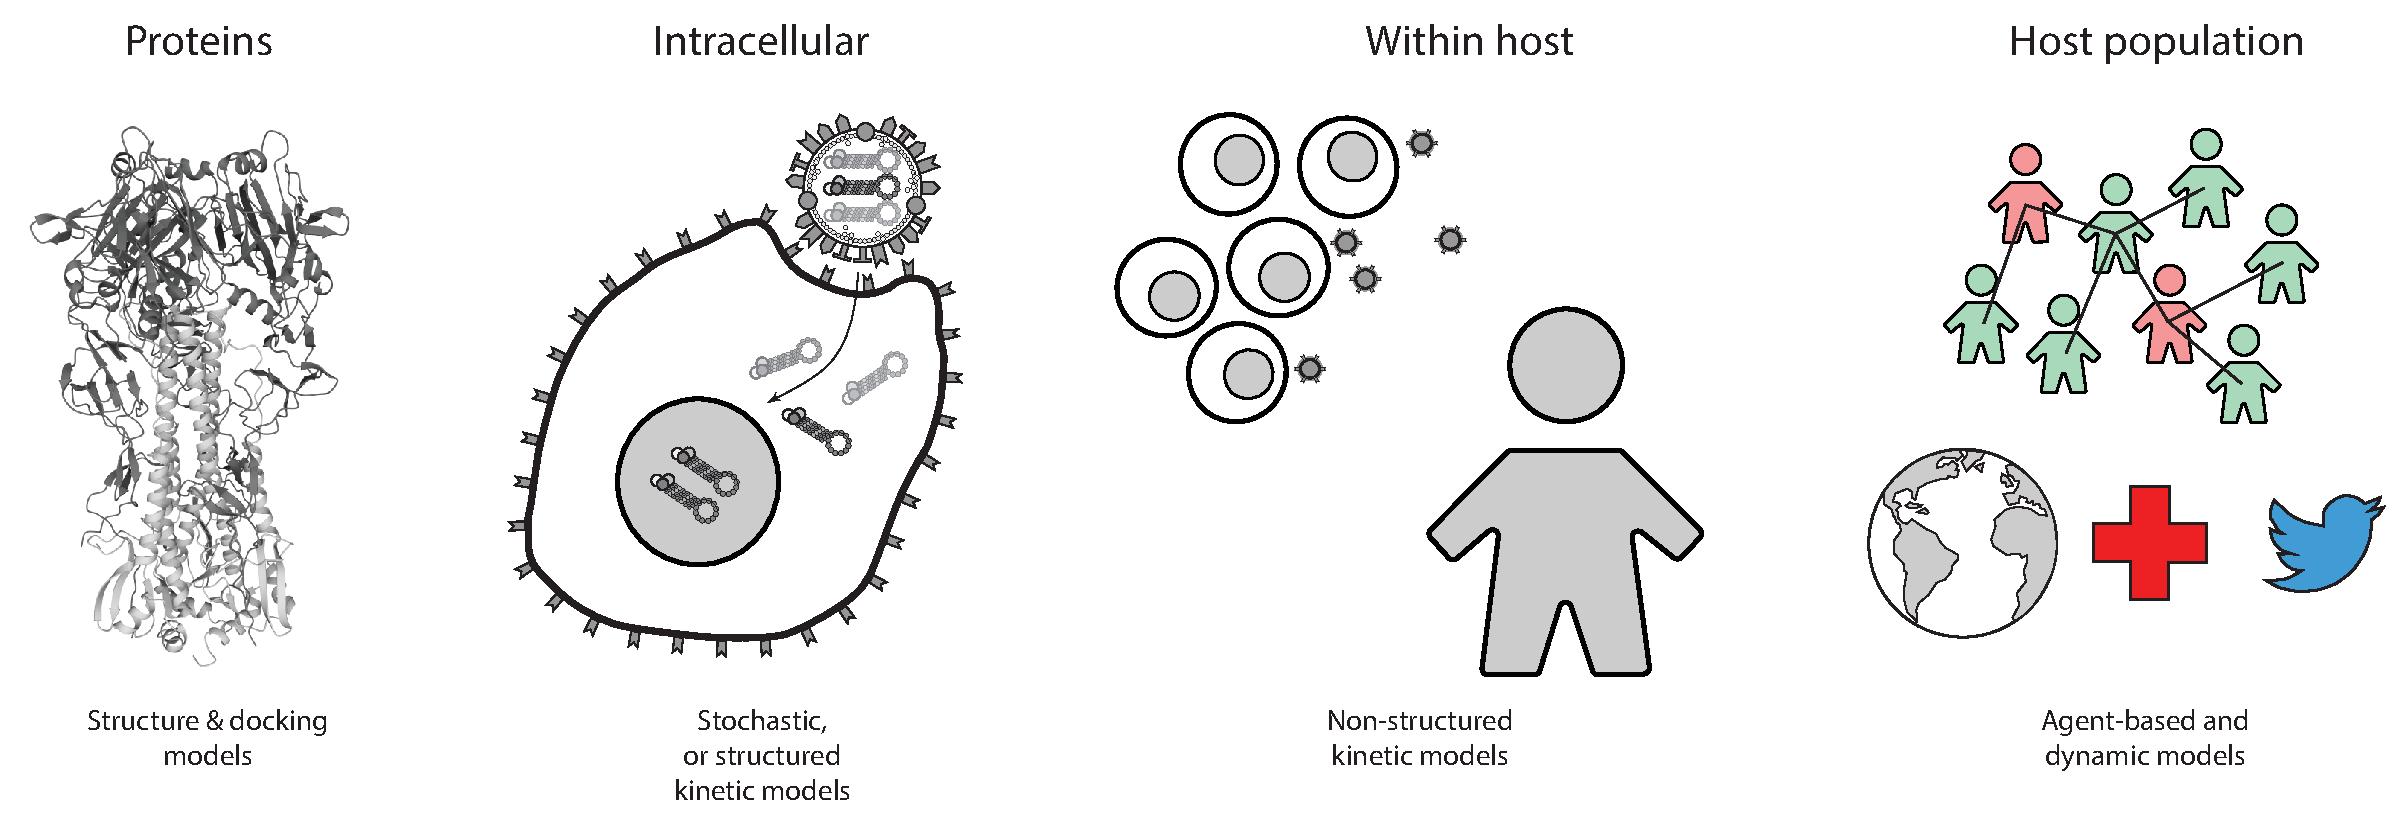
\includegraphics[width=1\textwidth, trim={0cm 0cm 0cm 0cm}, clip]{D_chapters/0_introduction/viralModelling copy.pdf}
\caption[Influenza computational modelling approaches on different scales]{Influenza computational modelling approaches on different scales. \par Hemagglutinin protein structure is a black and white render from \cite{influenzaVirusHemagglutininPDB}.}
\label{figure:modellingApproachesInfluenza}
\end{center}
\end{figure}

The knowledge of amino acid sequence and protein folding allow to predict the structure \cite{lin2007structure, russell2018influenza} of the viral proteins, and how they can bind to their targets or inhibitors \cite{li2015inhibitors, jagadesh2016influenza}.

On intracellular level, stochastic and structured kinetic approaches are used to model specific processes during the infection. Structured models which include individual processes in virus replication \cite{sidorenko2004structured}, endosomal escape \cite{lagache2012modeling} and defective viral particle propagation \cite{rudiger2019multiscale} have been proposed. Their phenomenological nature means that they often rely on unobserved quantities and variables, and do not allow for inference on specific molecular targets for intervention.

Non-structured kinetic models are used to describe the transmission within the host – cell culture or an individual. These models aim to understand and quantify the progression of the infection, and determine its resulting severity and duration \cite{beauchemin2008modeling}. We further discuss existing non-structured kinetic models and their applications in Chapter \ref{ch:DARPin}.

Finally, to describe the transmission between the hosts, dynamic or agent-based models are utilized. Influenza infection dynamic models focus primarily on transmission between hosts, with the goal of informing public health decisions and assist in pandemic planning \cite{ferguson2006strategies, mcvernon2007model}. With the advancement of social media, a new type of influenza forecasting models has emerged \cite{pawelek2014modeling, santillana2015combining, levy2018modeling}, relying on publicly available self-reporting by users. Agent-based models incorporate individual behavioral patterns to determine how social policies and educational efforts can affect viral spread within the population \cite{karimi2015effect}.

Despite the abundance of knowledge about influenza and its components, these approaches are used separately, and rarely make use of knowledge obtained through other methods, which makes mechanistic predictions about the underlying processes difficult. The reason for this is that combining these various levels of description in a meaningful manner is a non-trivial problem.


\section{Contributions of this thesis}

The goal of this thesis was to demonstrate the viability of a layered multiscale modelling approach for analysis of a complex biological system. Specifically, the biological system of choice is HDAC6-mediated influenza uncoating and consequent viral infection, in normal and perturbed conditions.

In Chapter \ref{ch:TugOfWar} we.

In Chapter \ref{ch:ReactionModels} we.

In Chapter \ref{ch:DARPin} we.

%\section{LaTeX examples}

\Citet{Maxwell1865} derived some very useful equations for electromagnetic
fields:
\begin{align}
    \nabla \cdot \vec{D} = \rho \\
    \nabla \cdot \vec{B} = 0 \\
    \nabla \times \vec{E} = -\frac{\partial \vec{B}}{\partial t} \\
    \nabla \times \vec{H} = \vec{j} + \frac{\partial \vec{D}}{\partial t}
\end{align}

The energy--momentum relation, \cref{eq:energy-momentum}, is one of \emph{my}
important results:
\begin{align}
    E^2 = m^2 c^4 + (p c)^2 \label{eq:energy-momentum}
\end{align}

Write units like this: \u{5}{\micro\meter}.

